\section{Introduction}
Retrieval-Augmented Generation (RAG)~\cite{REALM2020Guu,Retrieval2020Lewis,asai2023self,shi2023replug} has proven effective in mitigating hallucinations~\cite{elazar2021measuring,ji2023survey,shuster2021retrieval,huang2023survey} in Large Language Models (LLMs). RAG retrieves relevant knowledge from the knowledge base and incorporates the external information as the input context~\cite{Ram2023Incontextlearning}, benefiting various knowledge-intensive tasks~\cite{trivedi2023interleaving,izacard2022few,he2021efficient}. Existing studies typically employ automated evaluation metrics to assess the outputs of RAG systems during both training~\cite{rag-ddr2024Li} and evaluation~\cite{Radit2023Lin,Retrieval2023Gao} phases. These metrics primarily focus on string-level exact matching, which is less effective for determining whether the LLM-generated responses align with the ground truth~\cite{EnablingLargeLanguageModelstoGenerateTextwithCitations2023GaoTianyu,saad2024ares}, posing a challenge for RAG systems.

% !TEX root = main.tex

\begin{figure}[t]
\vspace{-1.5cm}
\begin{minipage}{0.34\textwidth}
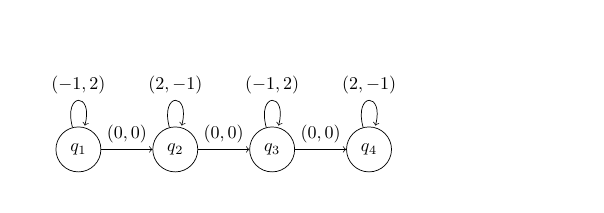
\begin{tikzpicture}[scale=0.25]
\usetikzlibrary{automata, positioning}
\scalebox{0.65}{
\node[state] (q1) {$q_1$};
\node[state, right=of q1] (q2) {$q_2$};
\node[state, right=of q2] (q3) {$q_3$};
\node[state, right=of q3] (q4) {$q_4$};

\path[->] (q1) edge [loop above] node[above] {$(-1,2)$} (q1) edge node[above] {$(0,0)$} (q2); 
\path[->] (q2) edge [loop above] node[above] {$(2,-1)$} (q2) edge node[above] {$(0,0)$} (q3);
\path[->] (q3) edge [loop above] node[above] {$(-1,2)$} (q3) edge node[above] {$(0,0)$} (q4);
\path[->] (q4) edge [loop above] node[above] {$(2,-1)$} (q4);
}
\end{tikzpicture}
\end{minipage}
\begin{minipage}{0.32\textwidth}
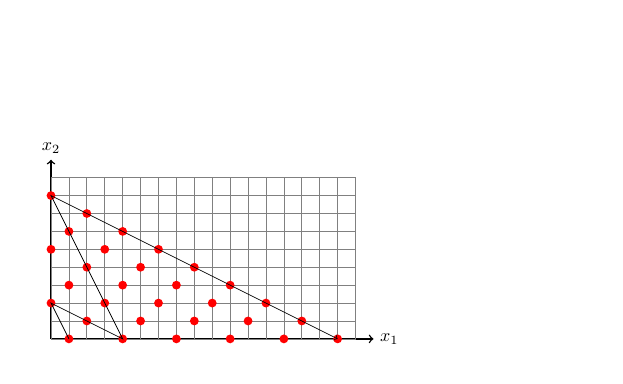
\begin{tikzpicture}[scale=0.35]
\scalebox{0.65}{
\draw[->, thick] (0, 0) -- (18, 0) node[right] {$x_1$};
\draw[->, thick] (0, 0) -- (0, 10) node[above] {$x_2$};

\draw[step=1, gray, thin] (0, 0) grid (17, 9);

\foreach \x in {1,4,7,10,13,16} \fill[red] (\x,0) circle (7pt);
\foreach \x in {2,5,8,11,14} \fill[red] (\x,1) circle (7pt);
\foreach \x in {0,3,6,9,12} \fill[red] (\x,2) circle (7pt);
\foreach \x in {1,4,7,10} \fill[red] (\x,3) circle (7pt);
\foreach \x in {2,5,8} \fill[red] (\x,4) circle (7pt);
\foreach \x in {0,3,6} \fill[red] (\x,5) circle (7pt);
\foreach \x in {1,4} \fill[red] (\x,6) circle (7pt);
\foreach \x in {2} \fill[red] (\x,7) circle (7pt);
\foreach \x in {0} \fill[red] (\x,8) circle (7pt);

\draw[->] (1,0) -- (0,2) -- (2,1) -- (4,0) -- (3,2) -- (2,4) -- (1,6) -- (0,8) -- (2,7) -- (4,6) -- (6,5) -- (8,4) -- (10,3) -- (12,2) -- (14,1) -- (16,0);
}
\end{tikzpicture}
\end{minipage}
\begin{minipage}{0.32\textwidth}
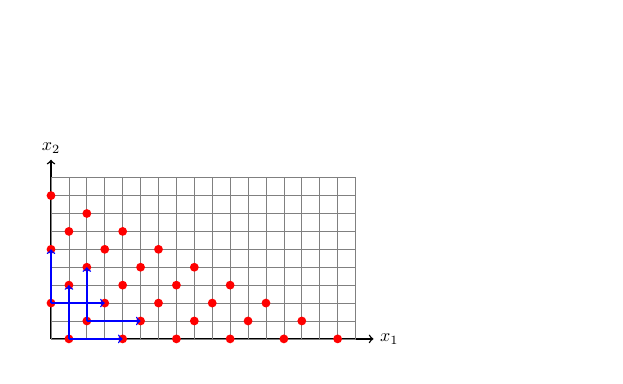
\begin{tikzpicture}[scale=0.35]
\scalebox{0.65}{
\draw[->, thick] (0, 0) -- (18, 0) node[right] {$x_1$};
\draw[->, thick] (0, 0) -- (0, 10) node[above] {$x_2$};

\draw[step=1, gray, thin] (0, 0) grid (17, 9);

\foreach \x in {1,4,7,10,13,16} \fill[red] (\x,0) circle (7pt);
\foreach \x in {2,5,8,11,14} \fill[red] (\x,1) circle (7pt);
\foreach \x in {0,3,6,9,12} \fill[red] (\x,2) circle (7pt);
\foreach \x in {1,4,7,10} \fill[red] (\x,3) circle (7pt);
\foreach \x in {2,5,8} \fill[red] (\x,4) circle (7pt);
\foreach \x in {0,3,6} \fill[red] (\x,5) circle (7pt);
\foreach \x in {1,4} \fill[red] (\x,6) circle (7pt);
\foreach \x in {2} \fill[red] (\x,7) circle (7pt);
\foreach \x in {0} \fill[red] (\x,8) circle (7pt);

\draw[->,blue,thick] (1,0) -- (4,0);
\draw[->,blue,thick] (1,0) -- (1,3);

\draw[->,blue,thick] (2,1) -- (5,1);
\draw[->,blue,thick] (2,1) -- (2,4);

\draw[->,blue,thick] (0,2) -- (3,2);
\draw[->,blue,thick] (0,2) -- (0,5);
}
\end{tikzpicture}
\end{minipage}
\caption{Left: 4-component \dvass $V_2$. 
Middle: the set $\reach_{q_4}(V_2, q_1(1,0))$ and a path $q_1(1,0) \tran q_4(16,0)$.
Right: bases 
%$A = \{(1,0),(2,1),(0,2)\}$ 
and periods 
%$P = \{(0,3),(3,0)\}$
 of an over-approximating semi-linear set $A+P^*$.}
\label{fig:zigzag}
\end{figure}

\begin{example}
For $k\geq 1$, let $V_k$ be a $(2k)$-component \dvass, where each component has just one state $q_i$
and one transition:
$(q_i, (-1,2), q_i)$ for odd $i$, and $(q_i, (2,-1), q_i)$ for even $i$.
Bridge transitions are $(q_i, (0,0), q_{i+1})$.
Figure~\ref{fig:zigzag} shows $V_2$ (left) and 
a path in $V_2$ from $s = q_1(1,0)$ to $t = q_4(16,0)$ together with 
the reachability set $\reach_{q_4}(V_2, s)$ (middle).
In general,
\begin{align} \label{eq:reachk}
X_k := \reach_{q_{2k}}(V_k, s) \ = \ \set{(x_1,x_2) \mid x_1+2x_2 \leq 4^k, \  x_1+2x_2 \equiv 1 \!\! \mod 3}.
\end{align}
Even if the size of the reachability set is 
exponential in $k$, for small $(x_1, x_2)$ it is periodic and the periods are small.
The set $X_k$ can be over-approximated by $A + P^*$ for $A = \set{(1,0),(2,1),(0,2)}$ and $P = \set{(0,3),(3,0)}$
(shown on the right of Figure~\ref{fig:zigzag}), namely for every $k\geq 1$ and $B\in\N$,
the set $X_k$ is \kanapka {$8$} {$B$}. 
For illustration, consider $Y := X_k \cap ((1,0) + P^*)$.
If $(1,0) + P^{\leq B} \subseteq X_k$ then $Y$ is a $B$-approximation
of $(1,0) + P^*$ with $\norm((1,0)), \norm(P) \leq 3 \leq 8$. 
Otherwise, there is some $(v_1, v_2) \in \big((1,0) + P^{\leq B}\big)\setminus X_k$, and
then $B$ is larger than $4^k$:
\[
%8B \geq 2(1 + 3B) \geq 2(v_1 + v_2) \geq v_1 + 2 v_2 > 
4^k < v_1 + 2 v_2 \leq 2(v_1 + v_2) \leq 2(1+3B) \leq 8B.
\]
Therefore by \eqref{eq:reachk}, each $(x_1,x_2) \in Y$ satisfies 
$\norm(x_1,x_2) = x_1 + x_2 \leq x_1 + 2x_2 \leq 4^k < 8B$, and thus
$Y$, seen as a union of singletons, is a union of 
linear sets with norm of base bounded by $8B$ and empty set of periods. 
In both cases, 
$Y$ is \kanapka {$8$} {$B$}. 
%The same intuition stays behind polynomial approximability of \dvass stated in Lemma~\ref{lem:2vass-sandwich}.
\end{example}


To enable more accurate evaluation of RAG models, some works incorporate LLMs as judgment models to assess the quality of generated responses~\cite{saad2024ares,friel2024ragbench,adlakha2023evaluating}, relying on their human-equivalent evaluation capabilities~\cite{chiang2023can,zheng2023judging,sottana2023evaluation}. These judgment models introduce specific evaluation dimensions, such as hallucination and comprehensiveness, to prompt LLMs to verify whether the generated responses align with the facts in the retrieved documents and whether all relevant information has been properly extracted and integrated~\cite{jin2024rag,jacovi2025facts,Rageval2024Zhu}. However, LLM-based judgment models are highly sensitive to the design of evaluation prompts~\cite{zhou2023survival,liu2024aligning}, which may lead to inconsistencies in judgments when different evaluation dimensions are employed.

In this paper, we introduce Judge-Consistency (\method{}), a method that enhances LLM-based judgment models to generate more accurate evaluations for RAG models in a self-improvement framework. \method{} incorporates specialized evaluation dimensions and employs a multiple-choice selection strategy for evaluation modeling. Additionally, \method{} leverages the Direct Preference Optimization (DPO) method~\cite{DPO2023Rafailov} to enhance the judgment capabilities of LLMs, while also implementing a ``judge as a judge'' mechanism during choosing preference pairs of judgments. Specifically, \method{} encourages LLMs to generate judgment results based on various combinations of judgment dimensions, evaluates the quality of these judgments using judge-consistency, and selects the chosen and rejected judgments for DPO training. This approach enhances the performance of the LLM-based judgment model without necessitating distillation from more powerful LLMs~\cite{zhang2025rag}.

Our experiments demonstrate the effectiveness of the \method{} method as a reward model for optimizing the RAG model, resulting in significant improvements over vanilla LLMs. Further analysis shows that \method{} helps LLMs select appropriate evaluation dimensions for assessing response quality by incorporating the agreements and consistency across different evaluation dimensions during optimization. Additionally, compared to other baselines, \method{} exhibits higher judgment consistency with the superior LLM, GLM-4-plus~\cite{du2022glm}, across various RAG evaluation datasets, further highlighting its effectiveness in optimizing LLMs to produce more accurate judgments on diverse RAG tasks.
% Our experiments demonstrate the effectiveness of \method{} method, achieving a improvement compared to baseline model. Further analysis reveals that this improvement stems from the judgment model, which aims to generate more accurate assessments to further optimize RAG models. Specifically, the judgment model is trained using \method{} method, enabling it to self-improve the evaluation performance without distillation from larger scale LLMs, and achieving more efficient gains at a lower cost.



% This process refines the judgment model by selecting the most appropriate evaluation dimensions, ultimately achieving more accurate assessments.


% designs four specific 
% utilizes the LLM itself to 

% error exposure model to generate high-quality reasoning errors that enhance the reasoning capabilities of LLMs. EULER utilizes the LLM itself as the error exposure model and applies the Direct Preference Optimization (DPO) method~\cite{rafailov2023direct} to train the exposure model to assign a higher probability to these LLM produced reasoning errors than the ground truth solutions. Subsequently, EULER employs the optimized error exposure model to generate erroneous reasoning examples for fine-tuning LLMs, while also providing valuable error examples within the prompt during inference. This approach guides LLMs in learning mathematical knowledge through errors and helps them avoid potential mistakes when solving mathematical problems.



% These models typically design prompts to instruct LLMs to determine whether the generated response aligns with the facts in the retrieved document and if all relevant information has been fully extracted and integrated~\cite{jin2024rag,jacovi2025facts,Rageval2024Zhu}. 




% when evaluating a RAG response based on whether it remains faithful to the context versus whether it contains redundant information, the LLM may produce different results.



% When LLMs use different evaluation dimensions to judge RAG responses, the judgments will be inconsistent. For example, for the given RAG responses, LLM judges it from two different evaluation dimensions, whether it is faithful to the context and whether it contains redundant information, respectively, which will produce different results. 

% avoid the significant costs and non-reproducibility of closed-source LLMs, some studies have turned to open-source as an alternative. 


% Besides, some studies have turned to open-source LLMs, such as LLaMA~\cite{touvron2023llama}, as alternatives



% However, calling the APIs of these closed-source models incurs high costs and reduces the reproducibility of evaluation results~\cite{SurveyonLLM-as-a-Judge2024Gu}. As a result, some studies have turned to open-source LLMs, such as LLaMA~\cite{touvron2023llama}, as an alternative. They fine-tune these open-source LLMs using the judgments generated by closed-source LLMs to bridge the gap in evaluation capabilities between them~\cite{wangpandalm,zheng2023judging}, which further extends the application scenarios of LLMs as the judgment models.

% Inspired by the success of LLMs as reward models in various tasks, RAG models also begin applying them to evaluate generated responses.



% To overcome this limitation, recent studies have explored the use of large language models as judges, leveraging their human-like understanding to evaluate generated responses. However, evaluation methods based on closed-source models come with high usage costs and low reproducibility. As a result, some researchers have turned to open-source models, such as LLaMA, as an alternative. They fine-tune these open-source models using evaluation results from closed-source models to bridge the gap in evaluation capabilities between the two.


% evaluating the responses of RAG systems remains a challenge. Automated evaluation metrics, such as exact match, typically focus on character-level similarity between the LLM-generated response and the ground truth, making them ineffective in assessing responses that are semantically correct but do not match the ground truth at the character level.








% Some approaches directly integrate vanilla LLMs into RAG systems to generate responses~\cite{izacard2022few}, but this may expose the model to noisy information, leading to factual errors. 







%challenge 1: evaluation提示设计敏感
%challenge 2: 闭源模型花费大,api背后模型升级导致不可复现
%优点 1: 不需要大量的标记数据
%优点 2: RAG中有很多维度,很敏感,容易出现bias. 我们的方法能缓解不一致性
%不同prompt影响很大,所以做一致性分析, 消除这个bias,用一致性提升
%引用格式再规范一下,缩写

%RAG怎么做,一笔带过
%丢进GPT里过一遍